\chapter{Testing with Original Data}

Here we will explore the results of different classifiers and active learning strategies on the original data. The original data consists of data discussed previously in Figure \ref{fig:original_english_counts} and shown discretely in the Attachments in Table \ref{tab:data_counts}. The original data was comprised of the original English and translated data but not the additionally collected data. 

\section{PWC, RBF Kernel, and Active Learning}

In our first experiment we used the radial bias function (RBF) kernel which is a popular kernel function. It is defined as:

\begin{equation}
    K(x_i, x_j) = \exp\left(- \frac{\left\| x_i - x_j \right\|^2}{2 \sigma^2}\right)
\label{eq:rbf_kernel}
\end{equation}

where $\sigma$ is a parameter that controls the smoothness of the kernel and $x_i$ and $x_j$ are the two points in the feature space to compare.

In Figure \ref{fig:plot_all_results_rbf} we have the train and test errors for four different active learning sampling strategies. XPAL appears to perform slightly better than PAL but not significantly better. We weren't satisfied with the testing error which plateaued around 70\%.

\begin{figure}[ht]
  \centering
  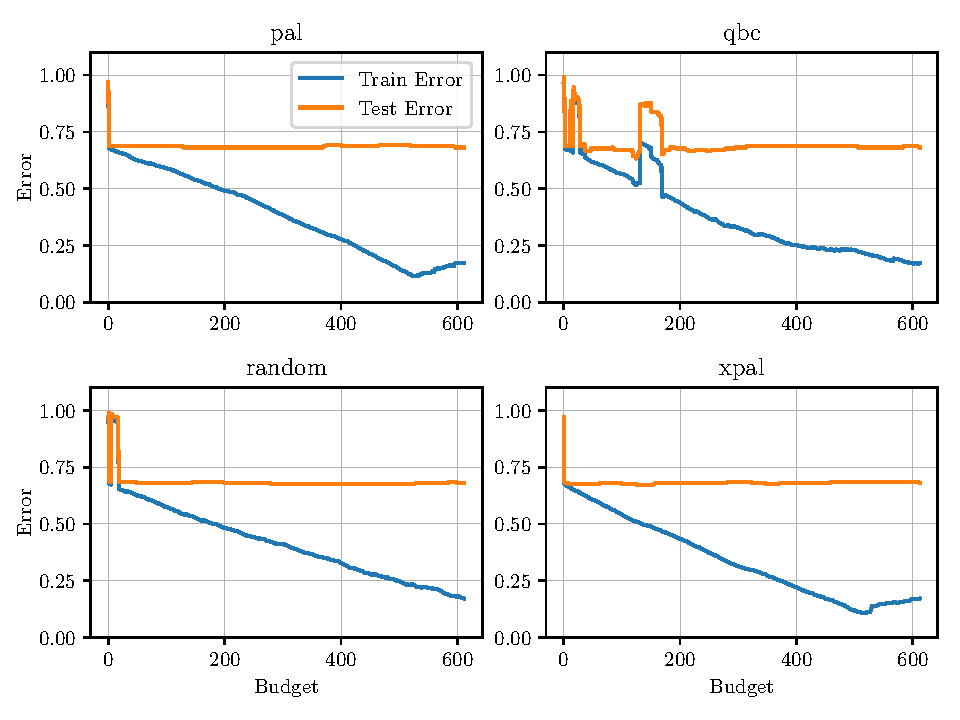
\includegraphics[width=\scale\textwidth]{../img/plot_all_results_rbf.pdf}
  \caption{Train and test error using different query strategies and RBF kernel for the PWC classifier.}
  \label{fig:plot_all_results_rbf}
\end{figure}

We later realized we made an error while constructing this experiment. While preparing data with the TF-IDF vectorizer we were fitting it using all the data instead of just the training data then transforming the test data. This resulted in the TF-IDF matrix having information about the test data so our error values are inaccurate. This fault was not fixed until the experiments in Section \ref{sec:classifier_evaluation}. However, we re-evaluated and re-ran a portion of the RBF and Cosine kernel experiments and obtained similar results to what was shown in Figures \ref{fig:plot_all_results_rbf} and \ref{fig:plot_all_results_cosine}.

\section{PWC, Cosine Kernel, and Active Learning}

In Figure \ref{fig:plot_all_results_cosine} we have the train and test errors for the same four different active learning sampling strategies tested on the same data. The only change was that we used Cosine kernel instead of the RBF kernel.The Cosine kernel is another important kernel function that is used in many machine learning algorithms. It is defined as:

\begin{equation}
    K(x_i, x_j) = \frac{x_i \cdot x_j}{\left\| x_i \right\| \left\| x_j \right\|}
\label{eq:cosine_kernel}
\end{equation}

where $x_i$ and $x_j$ are the two points in the feature space to compare. We found that we got better and more responsive results using the Cosine kernel in comparison to the RBF kernel.  

\begin{figure}[ht]
  \centering
  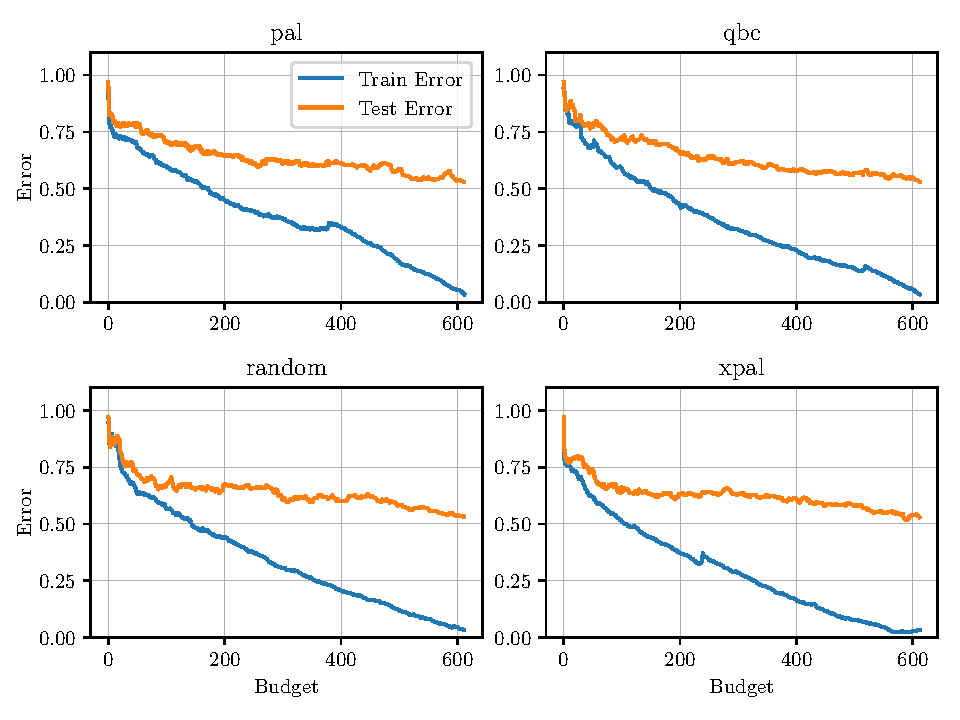
\includegraphics[width=\scale\textwidth]{../img/plot_all_results_cosine.pdf}
  \caption{Train and test error using different query strategies and Cosine kernel for the PWC classifier.}
  \label{fig:plot_all_results_cosine}
\end{figure}


In Figure \ref{fig:plot_all_results_cosine} it seemed that PAL and xPAL were able to reduce the training error, early in the training process compared to random selection and QBC. We also tested the other sampling strategies with the Cosine kernel and found that the results were similar. The other sampling strategies and their test data results are shown in Figure \ref{fig:cos_test_results} along with the test data from Figure \ref{fig:plot_all_results_cosine}. 


\begin{figure}[ht]
    \centering
    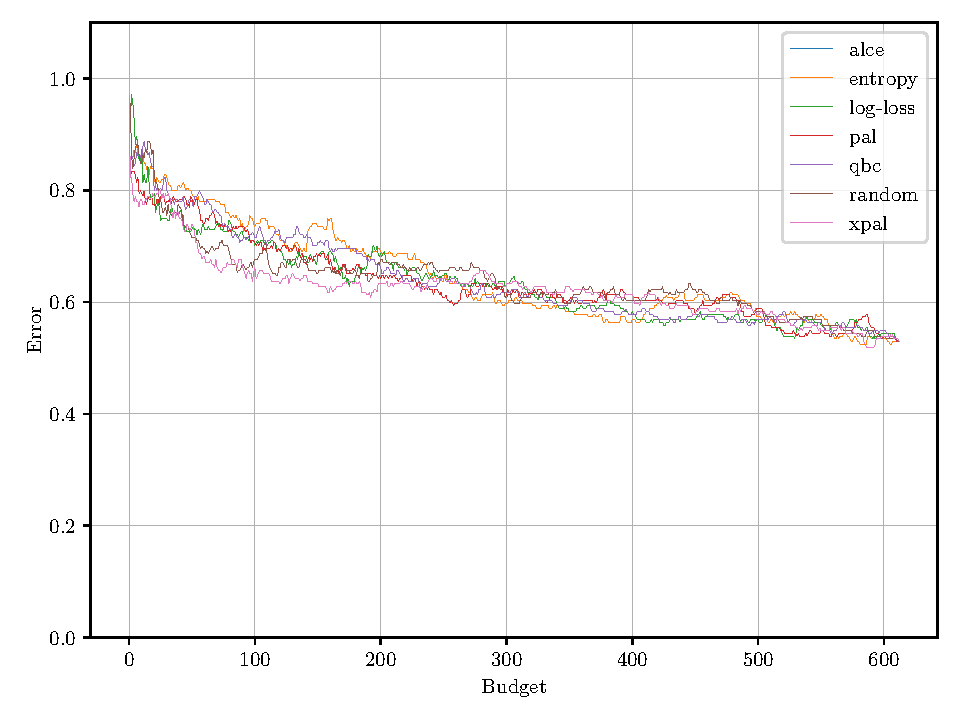
\includegraphics[width=\scale\textwidth]{../img/plot_kernel_cos_test_results.pdf}
    \caption{Comparing test error with one data split using different query strategies and Cosine kernel for the PWC classifier.}
    \label{fig:cos_test_results}
\end{figure}

We can see that the sampling strategies test performance converges over time (as we are using the same data and classifier). XPAL appears to be performing well early on in the training process, in the 100-200 budget range. This test is only showing the results of one data split. We can get a better idea if we run more tests with different train-test splits and average the results.

Figure \ref{fig:cos_test_results} shows that xPAL seems to be performing the best with our data but we wanted to see if we ran more tests with different train-test splits how the results would average out and which sampling strategy would perform the best on average. We ran 10 different data splits with each of the 7 sampling strategies and then took the average to get a smoother curve compared to the single run results shown in Figure \ref{fig:cos_test_results}. The results for this experiment are shown in Figure \ref{fig:cos_avg_test_results}. 

\begin{figure}[ht]
    \centering
    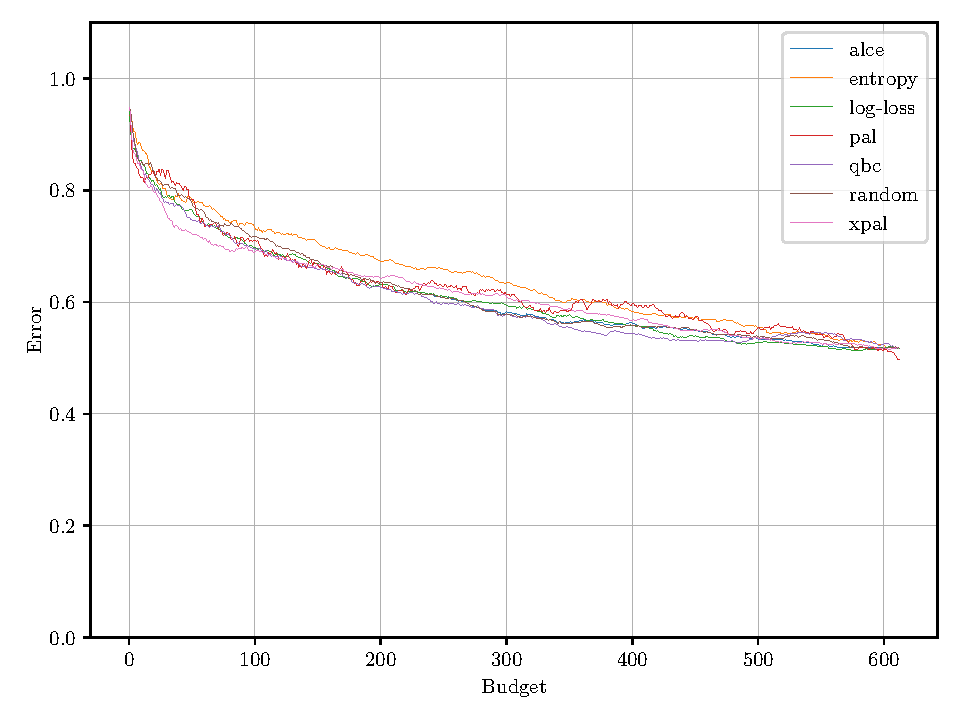
\includegraphics[width=\scale\textwidth]{../img/plot_kernel_cos_averaged_test_results.pdf}
    \caption{Comparing test error using different query strategies and Cosine kernel for the PWC classifier with results averaged over ten different data splits.}
    \label{fig:cos_avg_test_results}
\end{figure}

It is clear in Figure \ref{fig:cos_avg_test_results} that xPAL is performing the best early on (budget from 0-100) in the sample selection process. XPAL selects the data that minimizes the test error and builds the strongest classifier quickly while it takes the other sampling strategies more to get to the same level of performance. Around the 100 budget mark we can see that the other selection strategies catch up to xPAL performance wise. We want to note that for each plot where we averaged query strategies (10 runs/ splits per query strategy) that it took 24 hours on average to run the experiment on a CPU cluster, with PAL taking the longest of any of the sampling strategies.

\clearpage

\section{Classifier Evaluation}
\label{sec:classifier_evaluation}

We also decided to test out some classifiers from the Scikit-Learn library to compare performances. We used the original data with the proper TF-IDF vectorizer methodologies in all following chapters. It should be noted that cross validation was used here for evaluation but it was not used in the previous sections.

The goal of this exploratory phase was to try and decide which classifier to conduct more thorough testing with. As a result, we didn't use GridSearchCV for each classifier at this stage and we mostly used the default parameters and their cross validation scores with all of the original data (i.e. additional data not included). In some cases where using weights was an option for the classifier we included the precomputed Cosine decay weights. A table of the parameters used for each classifier is shown in the Attachments in Table \ref{tab:explore_classifiers_params}.

% THIS HAS BEEN FIXED
% Initially we made a minor error while evaluating the classifiers that used the precomputed weights in the following experiments. While computing the accuracy scores for the classifiers, we failed to incorporate the class weights that were used in training the classifier. This resulted in the accuracy scores being incorrectly calculated. This error persists throughout the rest of the experiments in this chapter up until the experiments in Section \ref{sec:proper_vectorization}.

The results for the different classifiers are shown in Figure \ref{fig:explore_classifiers}. In the box-plot, the whiskers extend from the box to the furthest data points that are within 1.5 times the inter-quartile range (IQR) of the box. Any data points that are beyond the whiskers are considered outliers and are plotted as individual points or symbols (diamonds) as seen in the figure.

\begin{figure}[ht]
  \centering
  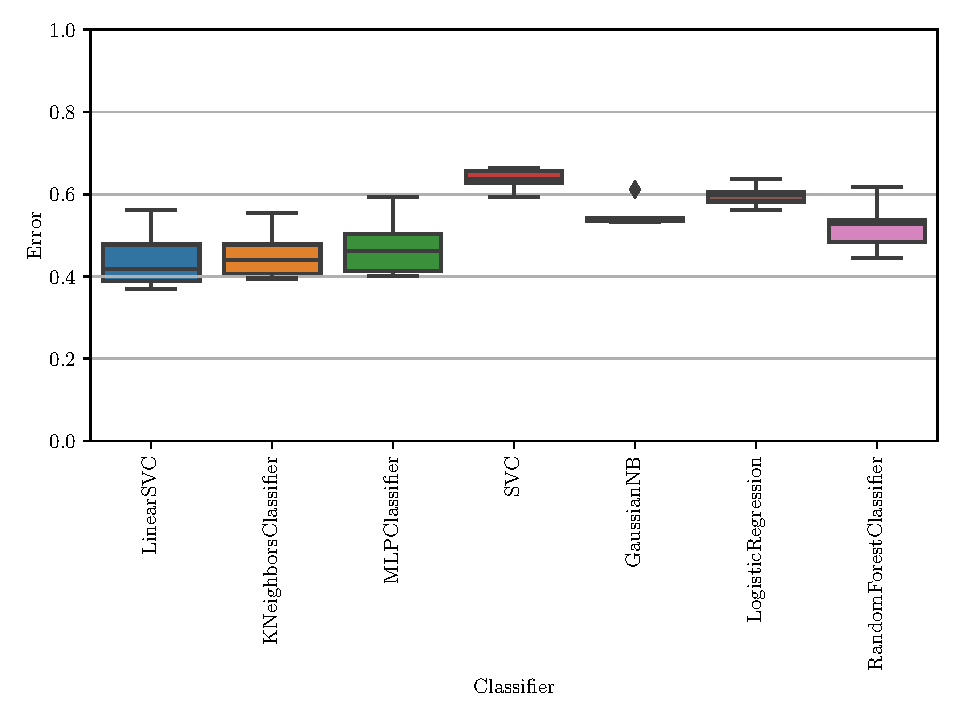
\includegraphics[width=\scale\textwidth]{../img/plot_explore_classifiers.pdf}
  \caption{Performance of base classifiers.}
  \label{fig:explore_classifiers}
\end{figure} 

The base LinearSVC classifier model performed best compared to other classifiers and it is a fast running algorithm even with data that has many features. We decided to look further into LinearSVC because it performed well. 

The LinearSVC is a type of machine learning algorithm that can be used for binary or multiclass classification problems. It's designed to predict one of two possible outcomes based on a set of input features. 

The basic idea behind the LinearSVC is to find the best line (or hyperplane) that can separate the two classes in the feature space. To do this, the algorithm looks for the line that maximizes the margin between the two classes. The margin is the distance between the decision boundary (i.e., the separating line) and the closest data points from each class. By maximizing the margin, the LinearSVC can achieve good generalization performance on new data.

In the case of multiclass classification, the LinearSVC works by dividing the data into multiple binary classification problems, one for each possible combination of classes. It then trains a separate binary classifier for each of these problems, which can then be used to classify new data points.

For example, if we have three classes A, B, C, then we have three classifiers, one for A versus B and C, one for B versus A and C, and another for C versus A and B. Once we have trained a separate LinearSVC for each binary classification problem, we can use them to classify new data points. To classify a new data point, we simply apply each binary classifier to the data point and see which classes it is predicted to belong to. If a data point is predicted to belong to more than one class, we can use a tie-breaking rule or simply choose the class with the highest predicted probability.

The LinearSVC algorithm seeks to find the hyperplane that maximally separates the classes in feature space, and weights are sometimes used that correspond to the coefficients of the hyperplane equation.

Consider another example using a binary classification problem where we have two classes labeled as -1 and +1. Given a set of training examples, the goal of the LinearSVC algorithm is to learn a hyperplane that separates the examples of the two classes in feature space. The hyperplane is defined by the equation:

\begin{equation}
w^T x + b = 0
\end{equation}

where w is a weight vector of the same dimension as the feature vectors x, and b is a bias term that shifts the hyperplane in the direction of the negative class.

During training, the LinearSVC algorithm tries to find the values of w and b that minimize the classification error while also maximizing the margin between the hyperplane and the closest examples of each class. This is achieved by solving a constrained optimization problem that involves minimizing the norm of the weight vector subject to the constraint that all training examples are correctly classified with a margin of at least 1.

Once the weights are learned, they can be used to make predictions on new examples by evaluating the sign of the decision function:

\begin{equation}
f(x) = w^T x + b
\end{equation}

If $f(x)$ is positive, the example is classified as the positive class, and if it is negative, the example is classified as the negative class. We created three different models using LinearSVC, the first was a boilerplate LinearSVC with no argument modifications, the second model used the class weights parameter set to 'balanced'. The 'balanced' mode uses the values of y to automatically adjust weights inversely proportional to class frequencies in the input data as $n\_samples / (n\_classes * np.bincount(y))$. 

For the third test we created a dictionary of weights for each class using the Cosine decay function. The weights for each category ranged from 0.1 to 1.0 where the most frequent classes had smaller weights. The Cosine decay function is defined as:

\begin{equation}
    w_i = \frac{1}{2} \left(1 + \cos \left(\frac{\pi t}{T}\right)\right)
\label{eq:cosine_decay}
\end{equation}

where $w_i$ is the weight for the $i^{th}$ class, $t$ is the current iteration, and $T$ is the total number of iterations. The Cosine decay function is a common function used for weights in machine learning algorithms. The calculated cosine weights are shown in the Attachments in Table \ref{tab:cosine_decay_weights}.

We used the same train test spilt for these experiments and the results for are shown in Table \ref{tab:lsvc_errors}. We also wanted to conduct more testing with KNeighborsClassifier and Neural Networks so created some small experiments to test these classifiers.

\begin{table}[!ht]
\centering
\caption{Test error for three different LinearSVC models using the original data.}
\begin{tabular}{lr}
\toprule
Model & Error \\
\midrule
No Weights & 0.382 \\
Balanced Weights & 0.402 \\
Cosine Decay Weights & 0.499 \\
\bottomrule
\end{tabular}

\label{tab:lsvc_errors}
\end{table}

Using K-Neighbors Classifier (KNN) and a Neural Network from TensorFlow we conducted additional tests. For the KNN we found that using 8 neighbors and the cosine distance metric yielded the lowest error. 

For the Neural Network we used a dense hidden-layer with 1000 neurons with Sigmoid activation and 23 output neurons with Softmax activation. For the NN optimizer we used Adamax with Cosine decay with an initial learning rate of 0.1, alpha value of 0.1 and 915 decay steps ($X\_data\_size // batch\_size * num_epochs$). The results are shown in Table \ref{tab:best_errors}. We can see that the K-Nearest Neighbors classifier and the Neural Network classifier performed slightly worse compared to LinearSVC.

The LinearSVC outperformed the other classifiers and we decided to experiment with it further. We attempted to boost performance of the LinearSVC classifier using multiple cross validation grid searches with bagging. Bagging (bootstrap aggregating) is a type of ensemble learning, where multiple models are trained on different subsets of the training data and their predictions are combined to make the final prediction. In Scikit-Learn we used the BaggingClassifier to implement bagging. An example of our setup and parameters are shown in the code snippet. 

\begin{verbatim}
    intercepts = np.linspace(0.1, 1, 20)
    c_vals = np.linspace(0.1, 1000, 20)
    base_classifier = LinearSVC(
        random_state=args.seed, 
        max_iter=10000)
    bagging_classifier = BaggingClassifier(
        base_estimator=base_classifier, 
        n_estimators=10, 
        random_state=args.seed)
    params = {
        'base_estimator__random_state': [args.seed],
        'base_estimator__intercept_scaling': 
            np.concatenate((intercepts, [1])),
        'base_estimator__loss': ['hinge', 'squared_hinge'],
        'base_estimator__penalty': ['l2'],
        'base_estimator__C': 
            np.concatenate((c_vals, [1])),
        'base_estimator__multi_class': 
            ['ovr', 'crammer_singer']
        }
    grid_search = GridSearchCV(
        estimator=bagging_classifier, 
        param_grid=params, 
        cv=5,
        scoring='accuracy',
        n_jobs=6)
\end{verbatim}

Performance was not improved from what we had already seen. Using bagging may not be the best approach at this stage because there are some categories that have very few samples so bagging may be unable to create a good model. We also didn't use the balanced class weights parameter because we had already seen that it was the worst performing class weight parameter in previous LinearSVC tests. The BaggingClassifier and GridSearchCV combination didn't improve the performance of the LinearSVC classifier beyond what we had already achieved.

\begin{table}[ht]
\centering
\caption{Test error for best performing classifiers using original data.}
\begin{tabular}{lr}
\toprule
                     Model &  Error \\
\midrule
                 LinearSVC &  0.382 \\
Tensor Flow Neural Network &  0.417 \\
    K Neighbors Classifier &  0.451 \\
\bottomrule
\end{tabular}

\label{tab:best_errors}
\end{table}

The precision-recall curve for the best performing classifier (LinearSVC) is shown in Figure \ref{fig:pr_curve} and the confusion matrix is shown in Figure \ref{fig:confusion_matrix} for the best performing LinearSVC classifier. The precision-recall curve gives us an idea at how well our classifier can correctly categorize the data. It also gives us a visualization of how unbalanced our categories are. We can see this imbalance clearly in Figure \ref{fig:pr_curve} where we have straight lines and large steps for some categories. This is a result of having a small number of data in a class. However, we can also see that for some classes the precision is relatively high even though we have few data points. Here we are namely concerned with the 'Culture' and 'Beauty' categories which have 10 and 31 data points respectively. It may be that the keywords in the 'Culture' and 'Beauty' categories are drastically different from the other categories so the performance is better. 

\begin{figure}[ht]
  \centering
  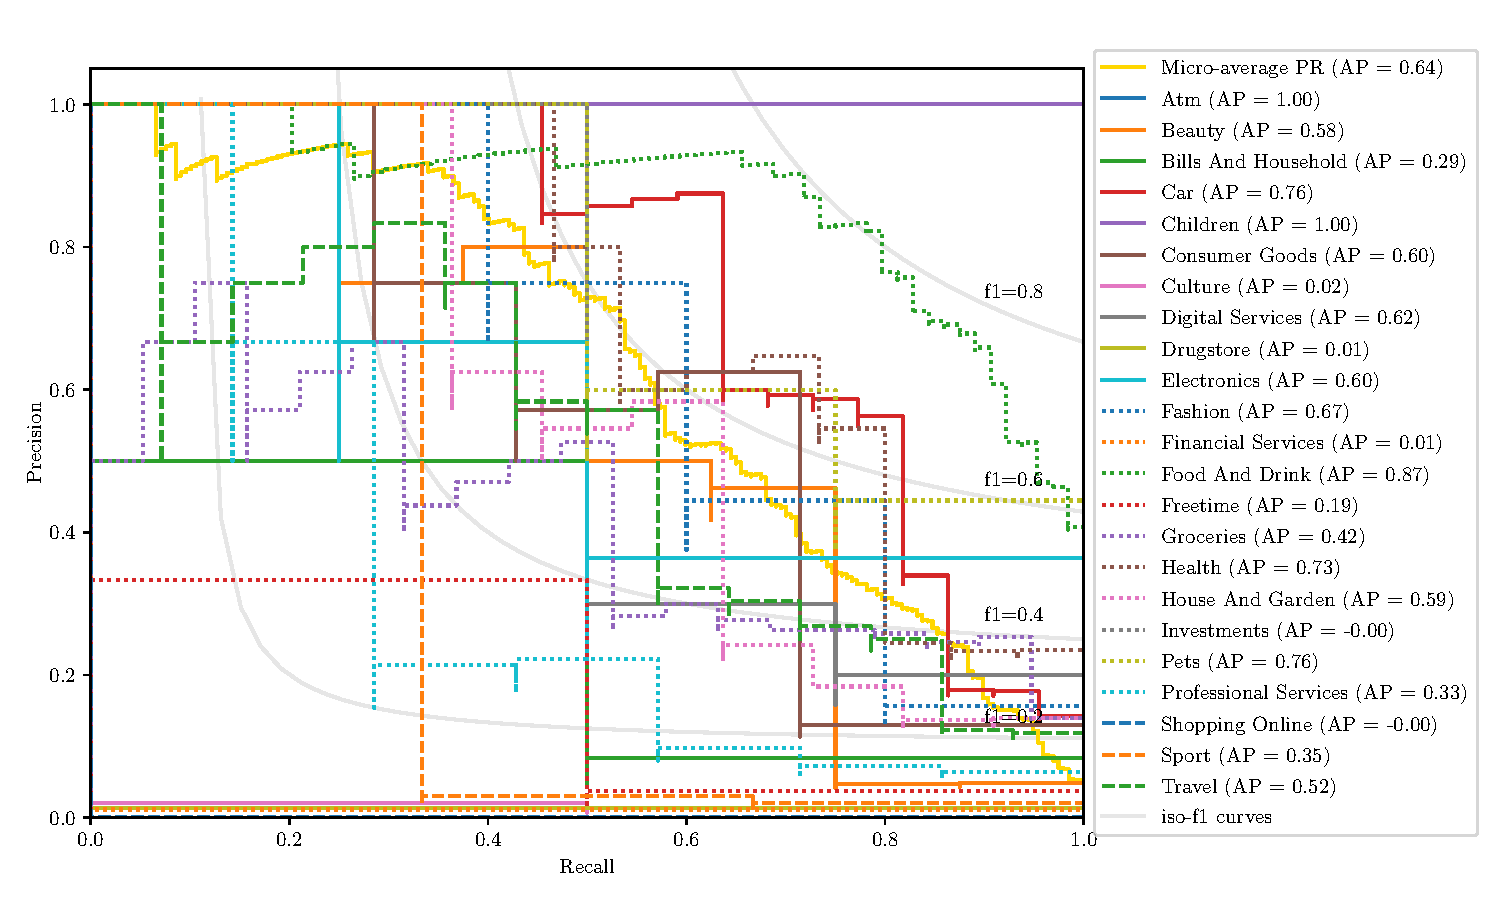
\includegraphics[width=\scale\textwidth]{../img/plot_pr_curve.pdf}
  \caption{Precision-recall curve for the best performing LinearSVC using the original data.}
  \label{fig:pr_curve}
\end{figure}

The confusion matrix shown in Figure \ref{fig:confusion_matrix} may be a better metric for visualizing this data. In addition, the classification report for the LinearSVC classifier is shown in the Attachments in Table \ref{tab:classification_report_LinearSVC} with F1, accuracy, precision, recall, and support scores.

\begin{figure}[ht]
  \centering
  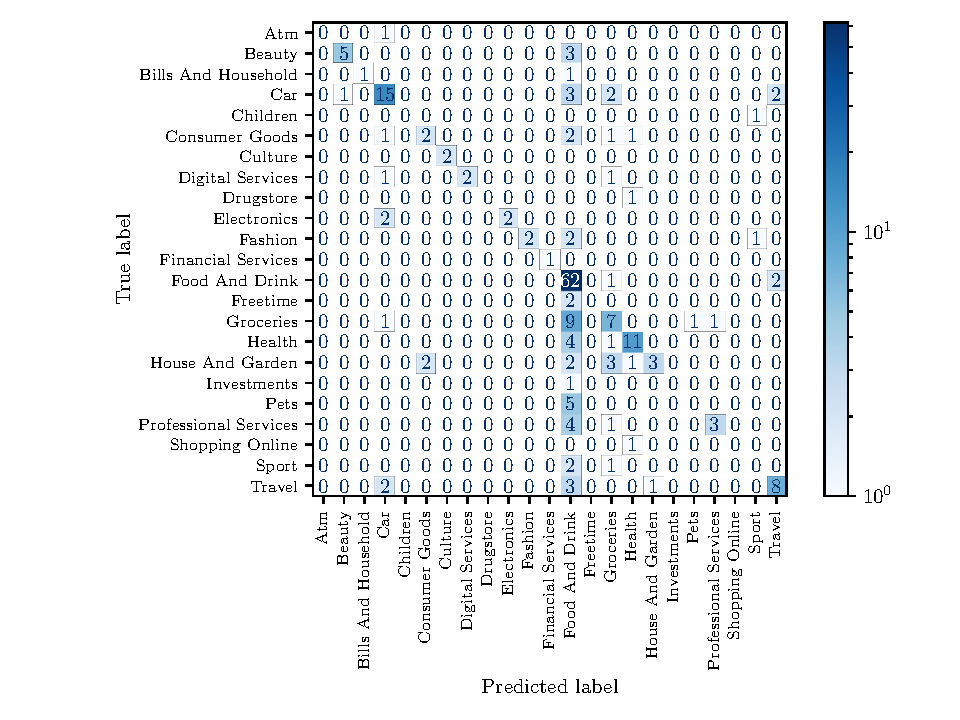
\includegraphics[width=\scale\textwidth]{../img/plot_cm_LinearSVC_original.pdf}
  \caption{Confusion matrix for the best performing LinearSVC classifier using the original data.}
  \label{fig:confusion_matrix}
\end{figure}


